\documentclass[12pt,oneside,a4paper,english]{article}
\usepackage{listings}
\usepackage{xcolor}
\usepackage[T1]{fontenc}
\usepackage{tikz}
\usepackage[margin=0.6in]{geometry}
\usepackage[font=small,labelfont=bf]{caption}

\def\checkmark{\tikz\fill[scale=0.4](0,.35) -- (.25,0) -- (1,.7) -- (.25,.15) -- cycle;} 

\lstset{
    language=SQL,
    basicstyle=\ttfamily,
    keywordstyle=\bfseries\color{blue},
    commentstyle=\color{gray},
    stringstyle=\color{green!60!black},
    morecomment=[l][\color{magenta}]{\#},
    moredelim=[s][\color{black}]{(}{)},
    morekeywords={TEXT, INTEGER},
}

\lstnewenvironment{bash}[1][]{
    \lstset{
        language=bash,
        basicstyle=\ttfamily\footnotesize,
        keywordstyle=\color{blue},
        commentstyle=\color{gray},
        stringstyle=\color{orange},
        showstringspaces=false,
        breaklines=true,
        frame=single,
        #1
    }
}{}

\title{Coursework Report}
\author{Constantinos Psaras}
\date{31/3/2024}
\newcommand{\username}{cp2n23}
\newcommand{\studentid}{35350172}


\begin{document}

\maketitle
\begin{center}
\section*{Personal Details}
\begin{tabular}{ll}
    Username: & \username \\
    Student ID: & \studentid \\
\end{tabular}
\end{center}
\newpage

\section*{Introduction}
This report presents the solutions to the coursework exercises.

\section{The Relational Model}
\subsection{EX1}


\small
 \begin{tabular}[t]{c c} % creating eight columns
  \hline\hline %inserting double-line
  \textbf{Relation} & \textbf{Type} \\ [0.3ex]
  \hline % inserts single-line
  dateRep - day & One-many\\ [0.3ex] 
  dateRep - month & One-many\\ [0.3ex]
  dateRep - year & One-many\\ [0.3ex]
  dateRep - cases & Many-many\\ [0.3ex]
  dateRep - deaths & Many-many\\ [0.3ex]
  dateRep - countriesAndTerritories & Many-many\\ [0.3ex]
  dateRep - geoId & Many-many\\ [0.3ex]
  geoId & Many-many\\ [0.3ex]
  dateRep - countryterritoryCode & Many-many\\ [0.3ex]
  dateRep - popData2020 & Many-many\\ [0.3ex]
  dateRep - continentExp & One-many\\ [0.3ex]
  day - month & Many-many\\ [0.3ex]
  day - year & Many-many\\ [0.3ex]
  day - cases & Many-many\\ [0.3ex]
  day - deaths & Many-many\\ [0.3ex]
  day - countriesAndTerritories & Many-many\\ [0.3ex]
  day - geoId & Many-many\\ [0.3ex]
  day - contryterritoryCode & Many-many\\ [0.3ex]
  day - popData2020 & Many-many\\ [0.3ex]
  day - continentExp & One-many\\ [0.3ex]
  month - year & Many-many\\ [0.3ex]
  month - cases & Many-many\\ [0.3ex]
  month - deaths & Many-many\\ [0.3ex]
  month - countriesAndTerritories & Many-many\\ [0.3ex]
  month - geoId & Many-many\\ [0.3ex]
  month - countryterritoryCode & Many-many\\ [0.3ex]
  month - popDat2020 & Many-many\\ [0.3ex]
  month - continentExp & One-many\\ [0.3ex]
  \hline
  \end{tabular}
  \begin{tabular}[t]{c c} % creating eight columns
  \hline\hline %inserting double-line
  \textbf{Relation} & \textbf{Type} \\ [0.3ex]
  \hline % inserts single-line
  year - cases & Many-many\\ [0.3ex]
  year - deaths & Many-many\\ [0.3ex]
  year - countriesAndterritories & Many-many\\ [0.3ex]
  year - geoId & Many-many\\ [0.3ex]
  year - countryterritoryCode & Many-many\\ [0.3ex]
  year - popData2020 & Many-many\\ [0.3ex]
  year - continentExp & One-many\\ [0.3ex]
  cases - deaths & Many-many\\ [0.3ex]
  cases - countriesAndTerriotories & Many-many\\ [0.3ex]
  cases - geoId & Many-many\\ [0.3ex]
  cases - countryterritoryCode & Many-many\\ [0.3ex]
  cases - popData2020 & Many-many\\ [0.3ex]
  cases - continentExp & One-many\\ [0.3ex]
  deaths - countrieAndTerritories & Many-many\\ [0.3ex]
  deaths - geoId & Many-many\\ [0.3ex]
  deaths - contryterritoryCode & Many-many\\ [0.3ex]
  deaths - popData2020 & Many-many\\ [0.3ex]
  deaths - continentExp &One-many\\ [0.3ex]
  countAndTerr - geoId & One-one\\ [0.3ex]
  countAndTerr - contryterritoryCode & One-one\\ [0.3ex]
  countAndTerr - popData2020 & One-one\\ [0.3ex]
  countAndTerr - continentExp & One-many\\ [0.3ex]
  geoId - countryterritoryCode & One-one\\ [0.3ex]
  geoId - popData2020 & One-one\\ [0.3ex]
  geoId - continentExp & One-many\\ [0.3ex]
  countterrCode - popData2020 & One-one\\ [0.3ex]
  countterrCode - continentExp & One-many\\ [0.3ex]
  popData2020 - continentExp & One-many\\ [0.3ex]
  \hline
\end{tabular}
\newpage
\begin{table}[h]
\centering
\begin{tabular}{|c|c|}
\hline
\textbf{Column Name} & \textbf{Data Type} \\ \hline
dateRep & TEXT \\ \hline
day & INTEGER \\ \hline
month & INTEGER \\ \hline
year & INTEGER \\ \hline
cases & INTEGER \\ \hline
deaths & INTEGER \\ \hline
countriesAndTerritories & TEXT \\ \hline
geoId & TEXT \\ \hline
countryterritoryCode & TEXT \\ \hline
popData2019 & INTEGER \\ \hline
continentExp & TEXT \\ \hline
\end{tabular}
\caption{Schema for the covidStats relation}
\label{tab:covidStats_schema}
\end{table}


\subsection{EX2}
\begin{center}
\begin{tabular}{|c|c|}
\hline
\textbf{Determinants} & \textbf{Determined} \\
\hline
day, month, year & dateRep \\
\hline
dateRep & day \\
\hline
dateRep, countriesAndTerritories & cases \\
\hline
dateRep & month \\
\hline
dateRep, countriesAndTerritories & deaths \\
\hline
dateRep & year \\
\hline
dateRep, countryterritoryCode & cases \\
\hline
dateRep, geoId & cases \\
\hline
dateRep, countryterritoryCode & deaths \\
\hline
dateRep, geoId & deaths \\
\hline
countriesAndTerritories & countryterritoryCode \\
\hline
geoId & countriesAndTerritories \\
\hline
countriesAndTerritories & continentExp \\
\hline
geoId & countryterritoryCode \\
\hline
countryterritoryCode & continentExp \\
\hline
countryterritoryCode & geoId \\
\hline
countriesAndTerritories & popData2020 \\
\hline
countryterritoryCode & popData2020 \\
\hline
geoId & continentExp \\
\hline
geoId & popData2020 \\
\hline
\end{tabular}
\end{center}

\textbf{Assumptions: }
\begin{itemize}
    \item The population of a country (\texttt{popData2020}) can not uniquely identify a country since some countries may have the same population.
    \item The \texttt{cases} and \texttt{deaths} attributes are either \texttt{null} or an integer value.
    \item The \texttt{day}, \texttt{month} and \texttt{year} attributes are not null.
    
\end{itemize}

\subsection{EX3}
\textbf{\large{Candidate Keys}}
\begin{enumerate}
    \item \textbf{\{dateRep, geoID\}}
    \item \textbf{\{dateRep, countriesAndTerritories\}}
    \item \textbf{\{dateRep, countriesAndTerritoriesCode\}}
    
\end{enumerate}
\subsection{EX4}
\begin{itemize}
\item Suitable primary keys would be \texttt{\{dateRep,geoID\}} or \texttt{\{dateRep,countryterritoryCode\}} or
\texttt{\{dateRep} \texttt{,countriesAndTerritories\}}. It makes most sense to use the country code, geographical ID or country name to uniquely identify each country. 
Out of the three \texttt{geoId} is the most suitable, as territories may later be added to \texttt{countriesAndTerritories}, making the field not unique for each country.
\item For the second part of the key using \texttt{dateRep} makes most sense, as the only other viable option would be using \texttt{day}, \texttt{month} and \texttt{year}.
\item Chosen Primary Key: \texttt{\{dateRep,geoID\}}
\end{itemize}

\section{Normalisation}
\subsection{EX5}
\begin{itemize}
    \item day, month, and year are functionally determined by dateRep. This indicates a partial-key dependency where non-prime attributes (day, month, year) are functionally determined by a subset of the candidate key (dateRep).

    \texttt{dateRep $\rightarrow$ day, month, year}
    
    Based on this partial-key dependency, we should decompose the relation into two additional relations(tables):
    \begin{itemize}
        \item Relation 1: \{dateRep, countriesAndTerritories, cases, deaths, geoId, countryterritoryCode, popData2020, continentExp\}
        \item Relation 2: \{dateRep, day, month, year\}

    \end{itemize}

    \item countriesAndTerritories, countryterritoryCode, continentExp and popData2020 are also functionally determined by geoId.

    \texttt{geoId $\rightarrow$ countriesAndTerritories, countryterritoryCode, continentExp, popData2020}

    We should therefore decompose this relation into two additional relations(tables):
    \begin{itemize}
        \item Relation 1: \{geoID ,dateRep,cases,deaths\}(Assuming we've already performed the first decomposition).
        \item Relation 2: \{geoID, countriesAndTerritories, countryterritoryCode, continentExp, popData2020\}
    \end{itemize}

    \item Third resulting relation: \texttt{geoId, dateRep $\rightarrow$ cases, deaths}
    

\end{itemize}

\subsection{EX6}
\begin{itemize}
    \item The introduction of 2 surrogate keys for \texttt{dateRep} and \texttt{geoId} named \texttt{date\_id} and \texttt{country\_id} respectively 
    \item The introduction of surrogate keys ensures data integrity against format changing of any of the fields.
    \item The two new surrogate keys now represent the primary keys of their respective relation.
    \item The resulting relations are:
    \begin{enumerate}
        \item \texttt{date\_id $\rightarrow$ dateRep, day, month, year}
        \item \texttt{country\_id $\rightarrow$ countriesAndTerritories, countryterritoryCode, \newline geoId, popData2020, continentExp}
        \item \texttt{date\_id, country\_id $\rightarrow$ cases, deaths}
    \end{enumerate}
\end{itemize}

\subsection{EX7}
\begin{itemize}
    \item Transitive dependencies occur when a non-prime attribute depends on another non-prime attribute rather than directly on the primary key.
    \item Identified Dependencies:

    
         \texttt{countriesAndTerritories $\rightarrow$ countryterritoryCode,countriesAndTerritories $\rightarrow$ continentExp, countryterritoryCode $\rightarrow$ continentExp}
         \texttt{geoId $\rightarrow$ continentExp, geoId $\rightarrow$ countriesAndTerritories, countriesAndTerritories $\rightarrow$ continentExp, geoId $\rightarrow$ countryterritoryCode,}
        \newline
        \texttt{countriesAndTerritories $\rightarrow$ countryterritoryCode}
\end{itemize}

\subsection{EX8}
\begin{itemize}
    \item 3NF Requirements:
    \begin{itemize}
        \item Each item in the relation contains only atomic values \checkmark
        \item Each attribute has a unique name \checkmark
        \item Order of rows does not matter \checkmark
        \item Each row must be unique \checkmark

        \item All non-key attributes must be fully functionally dependent on the entire primary key \checkmark

        \item There must exist no transitive dependencies \checkmark
    \end{itemize}
    \item All above dependencies contain prime attributes therefore there won't be any anomalies. Thus, the above relations are in 3NF.
\end{itemize}

\subsection{EX9}
\begin{itemize}
    \item Boyce-Codd Normal Form (BCNF) Requirements:
    \begin{itemize}
        \item Relation must be in 3NF \checkmark
        \item For every non-trivial functional dependency \textbf{X} $\rightarrow$ \textbf{Y} in the relation, \textbf{X} must be a superkey \checkmark
        \item Since no prime attributes are transitively dependent on a key, the above relations are already in BCNF
    \end{itemize}
\end{itemize}

\section{Modelling}
\subsection{EX10}
\begin{enumerate}
    \item \textbf{Navigate to database directory}
        
    \item \textbf{Launch SQLite}:
    Execute \texttt{sqlite3 coronavirus.db} to open the SQLite command-line interface and connect to the database.
        
    \item \textbf{Import data from csv file}:
    Use \texttt{.mode csv} and then \texttt{import dataset.csv dataset} to extract all data from the csv file.
        
    \item \textbf{Set output file and dump database}:
    Use \texttt{.output dataset.sql} to specify \texttt{dataset.sql} as the file to which the database dump will be written.
    Run \texttt{.dump} to populate \texttt{dataset.sql}.
\end{enumerate}



\subsection{EX11}
\begin{enumerate}
    \item \textbf{Create \texttt{ex11.sql}}: Normalize the database by creating additional tables with appropriate schema, indexes, and foreign keys, excluding the \texttt{dataset} table.
    
    \item \textbf{Dump Database}: Use SQLite command-line interface to dump the full database to \texttt{dataset2.sql}, capturing the schema and data. This ensures a complete backup of the database for easy restoration or transfer.
\end{enumerate}
\begin{lstlisting}
--Create countries table
CREATE TABLE IF NOT EXISTS countries (
	id INTEGER PRIMARY KEY AUTOINCREMENT NOT NULL,
	countriesAndTerritories TEXT NOT NULL UNIQUE,
	geoId TEXT UNIQUE,
	countryterritoryCode TEXT UNIQUE,
	popData2020 INTEGER NOT NULL,
	continentExp TEXT NOT NULL
);
--Create table dates
CREATE TABLE IF NOT EXISTS dates (
	id INTEGER PRIMARY KEY AUTOINCREMENT NOT NULL,
	dateRep TEXT NOT NULL UNIQUE,
	day INTEGER NOT NULL,
	month INTEGER NOT NULL,
	year INTEGER NOT NULL
);
--Create covidStats table
CREATE TABLE IF NOT EXISTS covidStats (
	date_id INTEGER,
	country_id INTEGER,
	cases INTEGER,
	deaths INTEGER,
	PRIMARY KEY (date_id, country_id),
	FOREIGN KEY (date_id) REFERENCES dates(id)
		ON DELETE CASCADE
		ON UPDATE NO ACTION,
	FOREIGN KEY (country_id) REFERENCES countries(id)
		ON DELETE CASCADE
		ON UPDATE NO ACTION
);
\end{lstlisting}


\subsection{EX12}
\begin{enumerate}
    \item \textbf{Create \texttt{ex12.sql}}:Populate the \texttt{covidStats}, \texttt{countries}, and \texttt{dates} tables by inserting data from the \texttt{dataset} table.
    \item \textbf{Dump Database}: Use SQLite command-line interface to dump the full database, including the populated tables, to \texttt{dataset3.sql}, capturing the schema and data. This ensures a complete backup of the database with the populated tables for easy restoration or transfer.
\end{enumerate}
\begin{lstlisting}
--Populate dates table
INSERT INTO dates SELECT DISTINCT NULL,dateRep,day,month,year FROM dataset;
--Populate countries table
INSERT INTO countries
SELECT DISTINCT NULL,
countriesAndTerritories,geoId,countryterritoryCode,popData2020,continentExp
FROM dataset;
--Populate covidStats table
-- Populate covidStats table, using COALESCE to handle NULL deaths
INSERT INTO covidStats (date_id, country_id, cases, deaths)
SELECT
    dates.id,
    countries.id,
    dataset.cases,
    CASE WHEN dataset.deaths = ''
        THEN 0
        ELSE CAST(dataset.deaths AS INTEGER)
        END AS deaths
FROM dataset
    INNER JOIN dates
        ON dates.dateRep = dataset.dateRep
    INNER JOIN countries
        ON countries.countriesAndTerritories = dataset.countriesAndTerritories;
\end{lstlisting}

\subsection{EX13}
Running \texttt{sqlite3 coronavirus.db < dataset.sql}, \texttt{sqlite3 coronavirus.db <ex11.sql}, \newline\texttt{sqlite3} \texttt{coronavirus.db < ex12.sql} succesfully re-generated the database.






\section{Querying}
\subsection{EX14}
\begin{itemize}
    \item Approach: Use \texttt{SUM} function to calculate total number of cases and deaths across all records in the covidStats table. Alias the sum as \texttt{total\_cases} and \texttt{total\_deaths} accordingly 

\item
\begin{lstlisting}
SELECT
    SUM(cases) AS total_cases,
    SUM(deaths) AS total_deaths
FROM covidStats;

\end{lstlisting}
\end{itemize}

\subsection{EX15}
\begin{itemize}
    \item Approach: Use \texttt{SELECT} statement to retrieve dateRep and cases columns from the covidStats table, filtering the records where geoId is \texttt{'UK'}. Order the results by dateRep in ascending order.

\item
\begin{lstlisting}
SELECT dateRep,cases
FROM covidStats
    INNER JOIN countries ON country_id=countries.id
    INNER JOIN dates ON date_id=dates.id
WHERE countries.countriesAndTerritories= 'United_Kingdom'
ORDER BY year,month,day;


\end{lstlisting}
\end{itemize}

\subsection{EX16}
\begin{itemize}
    \item Approach: \texttt{INNER JOIN} \texttt{countries} , \texttt{dates} and \texttt{covidStats} tables based on the surrogate keys.
    \item Select the date, cases, deaths and country name and order the results first by date and then by counttry name.

\item
\begin{lstlisting}
SELECT dateRep AS date,countriesAndTerritories AS countryName,cases,deaths
FROM covidStats
    INNER JOIN countries ON country_id=countries.id
    INNER JOIN dates ON date_id=dates.id
ORDER BY year,month,day, countryName;

\end{lstlisting}
\end{itemize}

\subsection{EX17}
\begin{itemize}
    \item Approach: Use \texttt{INNER JOIN} to join the \texttt{countries}  and \texttt{covidStats} tables based on the \texttt{country\_id}.
    \item Use the \texttt{SUM} function to aggregate the totals of both cases and deaths.
    \item Wrap the \texttt{SUM} with \texttt{ROUND} function to get the percentage in 2 decimal places.
\item
\begin{lstlisting}
SELECT
    countriesAndTerritories AS countryName,
    ROUND(SUM((cases * 100.0) / popData2020), 2)
        AS percent_cases_of_population,
    ROUND(SUM((deaths * 100.0) / popData2020), 2)
        AS percent_deaths_of_population
FROM
    covidStats
INNER JOIN
    countries ON country_id = countries.id
GROUP BY
    country_id;


\end{lstlisting}
\end{itemize}


\subsection{EX18}
\begin{itemize}
\item Approach: Use a \texttt{INNER JOIN} to joint \texttt{countries} and \texttt{covidStats} tables.
Group the entries by \texttt{countryName}
\item Order the results in descending order based on \texttt{percentDeaths} and \texttt{LIMIT} the results to 10 rows. 
\begin{lstlisting}
SELECT countriesAndTerritories AS countryName,
       ROUND((CAST(SUM(deaths) AS REAL) / NULLIF(SUM(cases), 0)) * 100, 2) 
           AS percentDeaths
FROM covidStats
    INNER JOIN countries ON country_id = countries.id
GROUP BY countryName
ORDER BY percentDeaths DESC
LIMIT 10;
\end{lstlisting}
\end{itemize}

\subsection{EX19}
\begin{itemize}
\item \texttt{INNER JOIN} the \texttt{countries}, \texttt{dates} and \texttt{covidStats} tables based on the corresponding surrogate keys.
\item Use \texttt{WHERE} to limit results to the UK.
\item Order the results chronologically 

\begin{lstlisting}
SELECT dateRep AS date,
       SUM(deaths) OVER (ROWS UNBOUNDED PRECEDING) AS cumulativeDeaths_UK,
       SUM(cases) OVER (ROWS UNBOUNDED PRECEDING) AS cumulativeCases_UK
FROM covidStats
    INNER JOIN countries ON country_id = countries.id
    INNER JOIN dates ON date_id = dates.id
WHERE countriesAndTerritories = 'Cyprus'
ORDER BY dateRep;
\end{lstlisting}
\end{itemize}


\newpage
\section{Extension}
\subsection{EX20}
\textbf{Script:}
\begin{bash}
#!/bin/bash

# Fetch the top 10 countries' IDs with the most deaths
IDS=$(sqlite3 coronavirus.db "SELECT country_id
                              FROM covidStats
                                  INNER JOIN countries ON country_id=countries.id
                              GROUP BY country_id
                              ORDER BY SUM(deaths) DESC
                              LIMIT 10;" | tr '\n' ' ')

# Fetch the names of the top 10 countries
NAMES=$(sqlite3 coronavirus.db "SELECT countriesAndTerritories
                                FROM covidStats
                                    INNER JOIN countries ON country_id=countries.id
                                GROUP BY country_id
                                ORDER BY SUM(deaths) DESC
                                LIMIT 10;" | tr '\n' ' ' |  tr '_' '-')

# Use gnuplot to generate the plot
gnuplot -persist <<-EOFMarker
  # Set plot settings
  set key top left autotitle columnheader
  set key reverse Left
  set title 'Cumulative COVID-19 Deaths Top 10'
  set ylabel 'Deaths'
  set xlabel 'Date'
  set grid
  set xdata time
  set datafile separator "|"
  set format x '%d/%m/%Y'
  set timefmt "%d/%m/%Y"
  set xtics mirror rotate by -45
  set rmargin at screen 0.94
  set term png
  set terminal png size 1024,768
  set output "graph1.png"

  # Set variables for country names and IDs
  titles = "$NAMES"
  ids = "$IDS"

  # Define function to retrieve country name from the titles variable
  ttl(n) = sprintf("%s", word(titles, n))

  # Plot data for each of the top 10 countries
  plot for [i=1:10] \
  '< sqlite3 coronavirus.db "SELECT dateRep,SUM(deaths) OVER (ROWS UNBOUNDED PRECEDING) FROM covidStats INNER JOIN countries ON country_id=countries.id INNER JOIN dates ON date_id=dates.id WHERE country_id='.word(ids, i).' ORDER BY year,month,day;"' \
   using 1:2 \
   title ttl(i) \
   w \
   l \
   lw 2
EOFMarker



\end{bash}

\newpage
\textbf{Result:}
\begin{figure}[h]
    \centering
    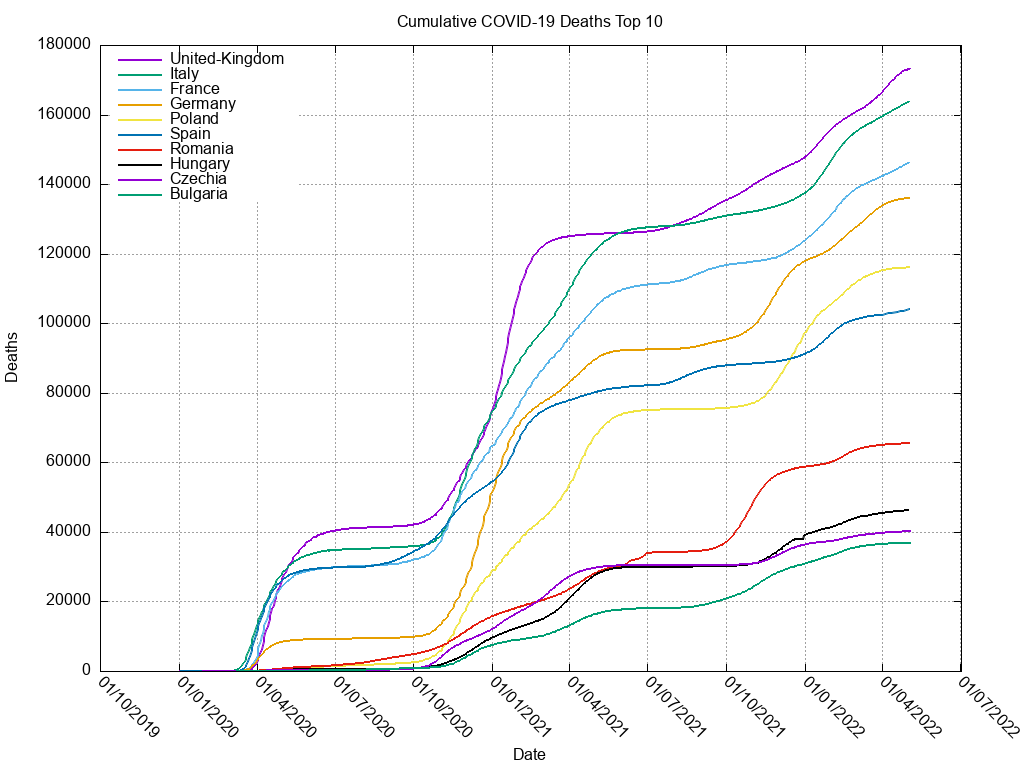
\includegraphics[width = 0.8\textwidth]{graph.png}
    \caption{Top 10 countries in terms of cumulative deaths}
    \label{fig:enter-label}
\end{figure}



\end{document}
